\section{Evaluation}
\label{section:evaluation}



\begin{table}[h]
\centering
\caption{Results of {\tool}, CVC4, and Z3/Z3str3 on Basic String Constraint benchmarks.}
\scalebox{0.85}{
\begin{tabular}{|l r | r r r r r|}
\hline
\multicolumn{2}{|c}{}                   & {\tool} & CVC4  &Z3 & Z3-str3 & Trau+  \\ \hline
\multirow{3}{*}{PyEx}		& SAT      & 19586*   & 20123 & 18490 &  3514 & 19149 \\ 
							& UNSAT    &  3858*   &  3841 &  3855 &  4521 & 3828 \\
							& $\times$ &  1977*   &  1457 &  3076 & 17386 & 2444 \\ \hline
\multirow{3}{*}{APLAS}		& SAT      &   128*   &    51 &    19 &    52 & 132 \\
							& UNSAT    &   287*   &   214 &   100 &   118 & 82 \\
							& $\times$ &   185*   &   335 &   481 &   430 & 386 \\ \hline
\multirow{3}{*}{LeetCode}	& SAT      &   856*   &   871 &   881 &   651 & 778 \\
							& UNSAT    &  1784*   &  1785 &  1785 &  1787 & 1827 \\
							& $\times$ &    26*   &    10 &     0 &   228 & 61 \\ \hline
\multirow{3}{*}{StringFuzz}	& SAT      &   502*   &   610 &   316 &   605 & 688 \\
							& UNSAT    &   294*   &   255 &   206 &   217 & 339 \\
							& $\times$ &   269*   &   200 &   543 &   243 & 38 \\\hline
\multirow{3}{*}{cvc4\textsubscript{pred}} & SAT & 16* & 11 &   12 &    10 & 247 \\
							& UNSAT    &   814*   &   818 &   807 &   778 & 500 \\
							& $\times$ &     5*   &     6 &    16 &    47 & 88 \\ \hline
\multirow{3}{*}{cvc4\textsubscript{term}} & SAT & 13* & 9 &     6 &    16 & 311 \\
							& UNSAT    &  1030*   &  1025 &  1020 &   962 & 596 \\
							& $\times$ &     2*   &    11 &    19 &    67 & 138 \\ \hline
\multirow{3}{*}{Total} 		& SAT      & 21101*  &  21675 & 19724 &  4848 & 21305  \\
							& UNSAT    &  8067*  &   7938 &  7773 &  8383 & 7172  \\
							& $\times$ &  2464*  &  2019 &   4135 & 18401 & 3155  \\\hline	
\end{tabular}}
\label{table:base_benchmark}
\end{table}

\begin{table}[h]
\centering
\caption{Results of {\tool}, CVC4, and Z3/Z3str3 on Basic String Constraints + String-Number Conversion benchmark.}
\scalebox{0.8}{
\begin{tabular}{|l r | r r r r|}
\hline
\multicolumn{2}{|c}{}                   			& {\tool} & CVC4   &    Z3  & Z3-str3 \\ \hline
\multirow{3}{*}{String-Number-Leetcode}	 & SAT      &   2356*  &  1766 &  1025  &   333 \\ 
										 & UNSAT    &  16369*  & 15612 & 17234  & 15543 \\
										 & $\times$ &    202*  &  1549 &   668  &  3051 \\ \hline 
\multirow{3}{*}{String-Number-PythonLib} & SAT      &    912*  &   586 &  1802  &   389 \\ 
										 & UNSAT    &    720*  &   666 &   744  &   729 \\
										 & $\times$ &   1014*  &  1394 &   100  &  1528 \\ \hline
\multirow{3}{*}{String-Number-JavaScript}& SAT      &     20   &     5 &    16  &     4 \\ 
										 & UNSAT    &      0   &     0 &     0  &     0 \\
										 & $\times$ &      0   &    15 &     4  &    16 \\ \hline \hline
\multirow{3}{*}{Total}					 & SAT      &   3288*  &  2357 &  2843  &   726 \\ 
										 & UNSAT    &  17089*  & 16278 & 17978  & 16272 \\
										 & $\times$ &   1216*  &  2958 &   772  &  4595 \\ \hline
\end{tabular}}
\label{table:str_int_benchmark}
\end{table}

\begin{table}[h]
\centering
\caption{Comparison of {\tool}, CVC4, and Z3/Z3str3 with checkLuhn problems of 2 to 12 loops.}
\scalebox{0.9}{
\begin{tabular}{| c | c c c c|}
\hline
\# of Loops & {\tool} 	  &  CVC4    	 &       Z3   & Z3-str3 \\ \hline
2 			& \textbf{SAT}(<0.1s)  &  \textbf{SAT}(0.27s)   & \textbf{SAT}(0.2s)  & $\times$ \\
3  			& \textbf{SAT}(<0.1s)  &  \textbf{SAT}(10.1s)  & \textbf{SAT}(0.1s)  & $\times$ \\
4 			& \textbf{SAT}(<0.1s)  &  \textbf{SAT}(48.7s) &   $\times$  & $\times$ \\
5 			& \textbf{SAT}(<0.1s)  &  $\times$     &   $\times$  & $\times$ \\
6 			& \textbf{SAT}(0.16s)  &  $\times$     & \textbf{SAT}(0.13s) & $\times$ \\
7 			& \textbf{SAT}(0.24s)  &  $\times$     &   $\times$  & $\times$ \\
8 			& \textbf{SAT}(0.31s)  &  $\times$     & \textbf{SAT}(0.37s) & $\times$ \\
9 			& \textbf{SAT}(0.26s)  &  $\times$     &   $\times$  & $\times$ \\
10 			& \textbf{SAT}(0.21s)  &  $\times$     & \textbf{SAT}(0.53s) & $\times$ \\
11 			& \textbf{SAT}(0.23s)  &  $\times$     & \textbf{SAT}(0.37s) & $\times$ \\
12 			& \textbf{SAT}(0.33s)  &  $\times$     & \textbf{SAT}(0.40s) & $\times$ \\ \hline
\end{tabular}}
\label{table:checkLuhn}
\end{table}


\hide{
\begin{figure}
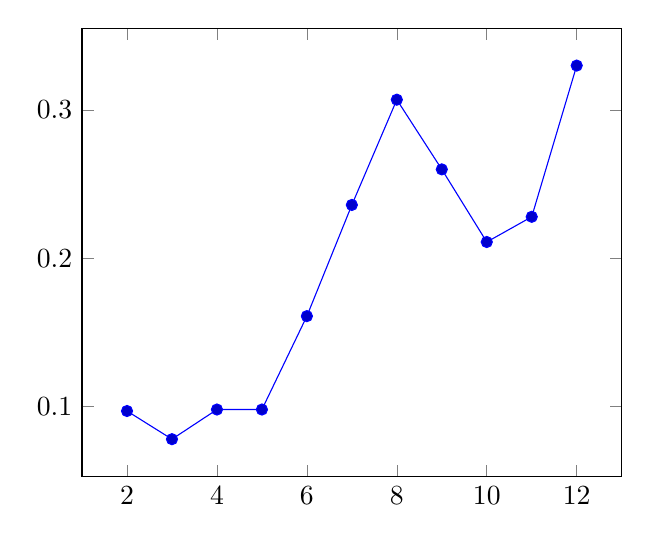
\begin{tikzpicture}
\begin{axis}
\addplot+[sharp plot]
coordinates
{
(2,0.097)
(3,0.078)
(4,0.098)
(5,0.098)
(6,0.161)
(7,0.236)
(8,0.307)
(9,0.26)
(10,0.211)
(11,0.228)
(12,0.33)
};
\end{axis}
\end{tikzpicture}
\caption{checkLuhn: z3-trau}
\end{figure}

\begin{figure}
\begin{tikzpicture}
\begin{axis}
\addplot+[sharp plot]
coordinates
{
(2,0.266)
(3,10.084)
(4,48.791)
(5,120)
(6,120)
(7,120)
(8,120)
(9,120)
(10,120)
(11,120)
(12,120)
};
\end{axis}
\end{tikzpicture}
\caption{checkLuhn: cvc4 (SAT if not timeout)}
\end{figure}

\begin{figure}
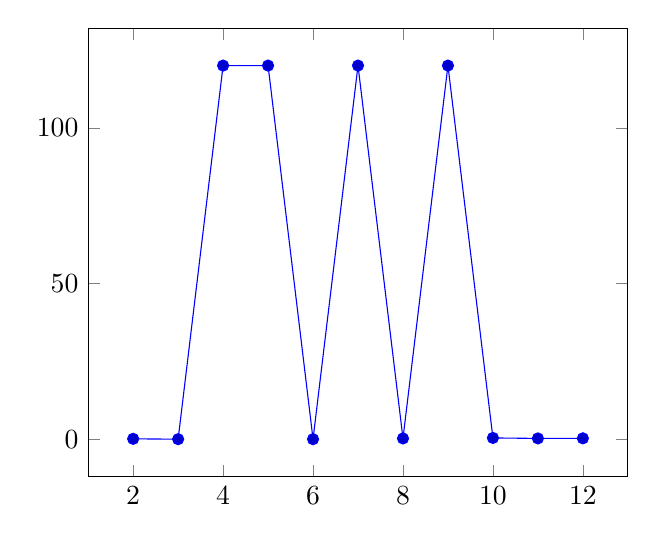
\begin{tikzpicture}
\begin{axis}
\addplot+[sharp plot]
coordinates
{
(2,0.238)
(3,0.128)
(4,120)
(5,120)
(6,0.134)
(7,120)
(8,0.366)
(9,120)
(10,0.526)
(11,0.374)
(12,0.405)
};
\end{axis}
\end{tikzpicture}
\caption{checkLuhn: z3 (SAT if not timeout)}
\end{figure}

\begin{figure}
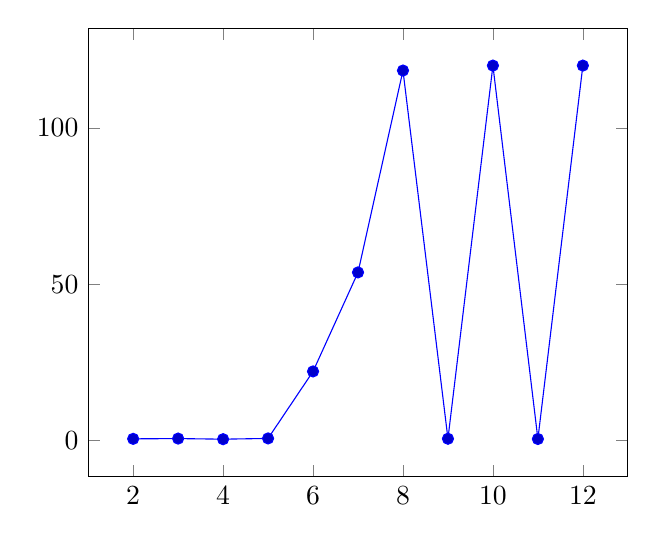
\begin{tikzpicture}
\begin{axis}
\addplot+[sharp plot]
coordinates
{
(2,0.4743)
(3,0.56052)
(4,0.36695)
(5,0.60905)
(6,22.06429)
(7,53.77536)
(8,118.41196)
(9,0.50559)
(10,120)
(11,0.42953)
(12,120)
};
\end{axis}
\end{tikzpicture}
\caption{checkLuhn: z3str3 (UNKNOWN if not timeout)}
\end{figure}
}


\hide{ % keep data of abc and ostrich
\begin{table}[h]
\centering
\caption{Results of Z3-Trau, CVC4, and Z3 on Basic String Constraint benchmarks (numbers with * will be updated later)}
\scalebox{0.7}{
\begin{tabular}{|l r | r r r r r r r|}
\hline
\multicolumn{2}{|c}{}                   & {\tool} & CVC4  &Z3 & Z3-str3 & Trau+ & ABC & Ostrich \\ \hline
\multirow{3}{*}{PyEx}		& sat      & 19586*   & 19763* & 18490 &   3024*  & 19149 & 0 & 111 \\ 
							& unsat    &  3858*   &  3834* &  3855 &   3839*  & 3828 & 0 & 871 \\
							& $\times$ &  1977*   &  1824* &  3076 &  18558*  & 2444 & 25421 & 24439 \\ \hline
\multirow{3}{*}{APLAS}		& sat      &   128*   &   205* &    19 &     38*  & 132 & 289 & 0 \\
							& unsat    &   287*   &   211* &   100 &    111*  & 82 & 2 & 1 \\
							& $\times$ &   185*   &   174* &   481 &    451*  & 386 & 309 & 599 \\ \hline
\multirow{3}{*}{LeetCode}	& sat      &   856*   &   860* &   881 &    670*  & 778 & 0 & 158 \\
							& unsat    &  1784*   &  1785* &  1785 &   1780*  & 1827 & 0 & 1618 \\
							& $\times$ &    26*   &    21* &     0 &    216*  & 61 & 2666 & 890 \\ \hline
\multirow{3}{*}{StringFuzz}	& sat      &   502*   &   677* &   316 &    493*  & 688 & 439 & 0 \\
							& unsat    &   294*   &   240* &   206 &    190*  & 339 & 158 & 0 \\
							& $\times$ &   269*   &   148* &   543 &    382*  & 38 & 468 & 1065 \\\hline
\multirow{3}{*}{cvc4\textsubscript{pred}} & sat & 16* & 11* &   12 &      8*  & 247 & 316 & 21 \\
							& unsat    &   814*   &   818* &   807 &    772*  & 500 & 443 & 17 \\
							& $\times$ &     5*   &     6* &    16 &     55*  & 88 & 76 & 797 \\ \hline
\multirow{3}{*}{cvc4\textsubscript{term}} & sat & 13* & 8* &     6 &     16*  & 311 & 576 & 45 \\
							& unsat    &  1030*   &   936* &  1020 &    958*  & 596 & 349 & 22 \\
							& $\times$ &     2*   &   101* &    19 &     71*  & 137 & 120 & 978 \\ \hline
\multirow{3}{*}{SLOG}  		& sat      & 0* & 1309* & 0 & 0* & 1228 & 1036 & 1299 \\
							& unsat    & 3391* & 2082* & 2824 & 2205* & 2079 & 1972 & 2079 \\
							& $\times$ & 0* & 0* & 567 & 1186* & 84 & 383 & 13 \\ \hline \hline
\multirow{3}{*}{Total} 		& sat      & * & * & 19724 & * &  &  &  \\
							& unsat    & * & * & 10597 & * &  &  &  \\
							& $\times$ & * & * &  4702 & * &  &  &  \\\hline
\end{tabular}}
\label{table:base_benchmark}
\end{table}
}


\hide{ %3rd version of tables
\begin{table}[t]
	\centering
	\caption{Results of {\tool}, cvc4, and z3 on str\_int benchmark (numbers with * will be updated later)}
	\scalebox{0.7}{
		\begin{tabular}{l r | r r r r}
			\hline
			\multicolumn{2}{c}{}                   & {\tool} & CVC4   &    Z3  & Z3-str3 \\ \hline
			\multirow{3}{*}{String-Number}		& sat      &   3294*  &  2185* &  2731* &    422* \\ 
			& unsat    &  17088*  & 16377* & 16832* &  16034* \\
			& $\times$ &   1191*  &  3011* &  2010* &   5117* \\ \hline \hline 
				
				\multirow{3}{*}{leetcode-addStrings}	& sat & 622*  &  330* &  100* &  85* \\ 
				& unsat    &  1054*  & 780* & 1043* &  634* \\
				& $\times$ &  2*  &  568* &  535* & 959* \\ \hline
				\multirow{3}{*}{leetcode-add\_Binary}	& sat & 520*  &  530* &  531* &  11* \\ 
				& unsat    &  1351*  & 1091* & 1091* &  1094* \\
				& $\times$ &  11*  &  261* &  260* & 777* \\ \hline
				\multirow{3}{*}{leetcode-numDecodings}	& sat & 166*  &  107* &  151* &  50* \\ 
				& unsat    &  273*  & 269* & 283* &  269* \\
				& $\times$ &  92*  &  155* &  97* & 212* \\ \hline
				\multirow{3}{*}{leetcode-restoreIpAddresses}	& sat & 811*  &  462* &  864* &  55* \\ 
				& unsat    &  13648*  & 13540* & 13648* &  13342* \\
				& $\times$ &  54*  &  511* &  1* & 1116* \\ \hline
				\multirow{3}{*}{leetcode-validIPAddress}	& sat & 54*  &  57* &  58* &  8* \\ 
				& unsat    &  19*  & 19* & 19* &  19* \\
				& $\times$ &  4*  &  1* &  0* & 50* \\ \hline
				\multirow{3}{*}{leetcode-validWordAbbreviation}	& sat & 183*  &  193* &  188* &  8* \\ 
				& unsat    &  24*  & 11* & 21* &  16* \\
				& $\times$ &  39*  &  42* &  37* & 222* \\ \hline
				\multirow{3}{*}{lib-datetime\_parse\_hh\_mm\_ss\_ff}	& sat &  133*  & 133* &  133* &  88* \\ 
				& unsat    &  41*  & 41* & 41* &  43* \\
				& $\times$ &  0*  &  0* &  0* & 43* \\ \hline
				\multirow{3}{*}{lib-datetime\_parse\_isoformat\_date}	& sat & 32*  &  32* &  32* &  23* \\ 
				& unsat    &  0*  & 0* & 0* &  0* \\
				& $\times$ &  0*  &  0* &  0* & 9* \\ \hline
				\multirow{3}{*}{lib-distutils\_get\_build\_version}	& sat & 19*  &  19* &  19* &  4* \\ 
				& unsat    &  24*  & 24* & 24* &  24* \\
				& $\times$ &  0*  &  0* &  0* & 15* \\ \hline
				\multirow{3}{*}{lib-email\_parsedate\_tz}	& sat & 68*  &  72* &  72* &  30* \\ 
				& unsat    &  138*  & 138* & 138* &  138* \\
				& $\times$ &  4*  &  0* &  0* & 42* \\ \hline
				\multirow{3}{*}{lib-http\_parse\_request}	& sat & 24*  &  24* &  24* &  8* \\ 
				& unsat    &  9*  & 9* & 9* &  7* \\
				& $\times$ &  0*  &  0* &  0* & 18* \\ \hline
				\multirow{3}{*}{lib-ipaddress\_ip\_int\_from\_string}	& sat & 595*  &  204* &  480* &  18* \\ 
				& unsat    &  427*  & 373* & 431* &  357* \\
				& $\times$ &  1006*  &  1451* &  1117* & 1653* \\ \hline
				\multirow{3}{*}{lib-nntplib\_parse\_datetime}	& sat & 4*  &  8* &  0* &  0* \\ 
				& unsat    &  0*  & 0* & 0* &  0* \\
				& $\times$ &  4*  &  0* &  8* & 8* \\ \hline
				\multirow{3}{*}{lib-smtpd\_parseargs}	& sat & 27*  &  27* &  27* &  24* \\ 
				& unsat    &  72*  & 72* & 72* &  66* \\
				& $\times$ &  0*  &  0* &  0* & 9* \\ \hline
				\multirow{3}{*}{lib-wsgiref\_check\_status}	& sat & 10*  &  10* &  10* &  6* \\ 
				& unsat    &  9*  & 9* & 9* &  9* \\
				& $\times$ &  0*  &  0* &  0* & 4* \\ \hline
				% \multirow{4}{*}{filtered\_str\_int}	& sat      &   3281*  &  2210* &  2729* &    424* \\
				% 									& unsat    &   2912*  &  2211* &  2655* &   1944* \\
				% 									& $\times$ &   1203*  &  2975* &  2012* &   5028* \\ \hline
			}
		\end{tabular}
		\label{table:str_int_benchmark}
	\end{table}
}

\hide{  % 2nd version of tables
\begin{table*}[t]
\centering
\caption{Results of {\tool}, cvc4, and z3 on string benchmarks (numbers with * will be updated later)}
\begin{tabular}{l r | r r r r r r r}
\hline
\multicolumn{2}{c}{}                   & {\tool} & CVC4  &    Z3 & Z3-str3 & Trau+ & ABC & Ostrich \\ \hline
\multirow{4}{*}{PyEx}		& sat      & 19586*   & 19763* & 18359 &   3024*  & 19149 & 0 & 111 \\ 
							& unsat    &  3858*   &  3834* &  3851 &   3839*  & 3828 & 0 & 871 \\
							& timeout  &  1969*   &     0* &  3211 &  16708*  & 2444 & 0 & 44 \\
							& $\times$ &     8*   &  1824* &     0 &   1850*  & 0 & 25421 & 24395 \\ \hline
\multirow{4}{*}{APLAS}		& sat      &   128*   &   205* &    19 &     38*  & 132 & 289 & 0 \\
							& unsat    &   287*   &   211* &   100 &    111*  & 82 & 2 & 1 \\
							& timeout  &   185*   &   174* &   481 &     93*  & 386 & 308 & 0 \\
							& $\times$ &     0*   &     0* &     0 &    358*  & 0 & 1 & 599 \\ \hline
\multirow{4}{*}{LeetCode}	& sat      &   856*   &   860* &   881 &    670*  & 778 & 0 & 158 \\
							& unsat    &  1784*   &  1785* &  1785 &   1780*  & 1827 & 0 & 1618 \\
							& timeout  &    26*   &    21* &     0 &     83*  & 15 & 0 & 0 \\
							& $\times$ &     0*   &     0* &     0 &    133*  & 46 & 2666 & 890 \\ \hline
\multirow{4}{*}{StringFuzz}	& sat      &   502*   &   677* &   311 &    493*  & 688 & 439 & 0 \\
							& unsat    &   294*   &   240* &   205 &    190*  & 339 & 158 & 0 \\
							& timeout  &   267*   &    63* &   549 &    377*  & 29 & 297 & 0 \\
							& $\times$ &     2*   &    85* &     0 &      5*  & 9 & 171 & 1065 \\ \hline
\multirow{4}{*}{cvc4\textsubscript{pred}} & sat & 16* & 11* &   12 &      8*  & 247 & 316 & 21 \\
							& unsat    &   814*   &   818* &   808 &    772*  & 500 & 443 & 17 \\
							& timeout  &     5*   &     6* &    15 &     41*  & 23 & 0 & 0 \\
							& $\times$ &     0*   &     0* &     0 &     14*  & 65 & 76 & 797 \\ \hline
\multirow{4}{*}{cvc4\textsubscript{term}} & sat & 13* & 8* &     6 &     16*  & 311 & 576 & 45 \\
							& unsat    &  1030*   &   936* &  1022 &    958*  & 596 & 349 & 22 \\
							& timeout  &     2*   &    12* &    17 &     53*  & 50 & 0 & 0 \\
							& $\times$ &     0*   &    89* &     0 &     18*  & 87 & 120 & 978 \\ \hline
\multirow{4}{*}{SLOG}  		& sat      & 0* & 1309* & 0 & 0* & 1228 & 1036 & 1299 \\
							& unsat    & 3391* & 2082* & 0 & 2205* & 2079 & 1972 & 2079 \\
							& timeout  & 0* & 0* & 631 & 1186* & 84 & 361 & 9 \\
							& $\times$ & 0* & 0* & 2760 & 0* & 0 & 22 & 4 \\ \hline
\end{tabular}
\label{table:base_benchmark}
\end{table*}

\begin{table*}[t]
\centering
\caption{Results of {\tool}, cvc4, and z3 on str\_int benchmark (numbers with * will be updated later)}
\begin{tabular}{l r | r r r r r r r}
\hline
\multicolumn{2}{c}{}                           & {\tool} & CVC4   &    Z3  & Z3-str3 & Trau+ & ABC & Ostrich \\ \hline
\multirow{4}{*}{full\_str\_int}		& sat      &   3294*  &  2185* &   422* &   2731* & 158 & 0 & 47 \\ 
									& unsat    &  17088*  & 16377* & 16034* &  16832* & 1609 & 0 & 213 \\
									& timeout  &   1191*  &  3011* &  4131* &   2010* & 439 & 0 & 144 \\
									& $\times$ &      0*  &     0* &   986* &      0* & 19367 & 21573 & 21169 \\ \hline
\multirow{4}{*}{filtered\_str\_int}	& sat      &   3281*  &  2210* &  2729* &    424* & 159 & 0 & 47 \\
									& unsat    &   2912*  &  2211* &  2655* &   1944* & 70 & 0 & 0 \\
									& timeout  &   1203*  &  2975* &  2012* &   4106* & 475 & 0 & 119 \\
									& $\times$ &     0*   &     0* &     0* &    922* & 6492 & 7396 & 7230 \\ \hline
\end{tabular}
\label{table:str_int_benchmark}
\end{table*}
}





\hide{  % 1st version of tables
\begin{table*}[t]
\centering
\caption{Results of {\tool}, cvc4, and z3 on string benchmarks}
\begin{tabular}{l | r r r | r r r | r r r | r r r}
\hline
\multirow{2}{*}{}   & \multicolumn{3}{|c|}{z3-Trau} & \multicolumn{3}{|c}{cvc4} & \multicolumn{3}{|c}{z3} & \multicolumn{3}{|c}{z3-str3} \\
			& sat & unsat & timeout/$\times$ & sat & unsat & timeout/$\times$ & sat & unsat & timeout/$\times$ & sat & unsat & timeout/$\times$ \\ \hline
PyEx		& 19586 & 3858 & 1969/8 & 19763 & 3834 & 0/1824 & 16581 & 3832 & 5008/0 & 3024 & 3839 & 16708/1850 \\ 
APLAS		&   128 &  287 &  185/0 & 205 &  221 & 174/0 &  13 &  100 & 486/1 & 38 & 111 & 93/358 \\ 
LeetCode	&   856 & 1784 &   26/0 & 860 & 1785 &  21/0 & 881 & 1785 & 0/0 & 670 & 1780 &  83/133 \\ 
StringFuzz	& 502 & 294 & 267/2 & 677 & 240 & 63/85 & 265 & 187 & 609/4 & 493 & 190 & 377/5 \\ 
cvc4\textsubscript{pred}	& 16 & 814 & 5/0 & 11 & 818 & 6/0 & 12 & 808 & 15/0 & 8 & 772 & 41/14 \\ 
cvc4\textsubscript{term}	& 13 & 1030 & 2/0 & 8 & 936 & 12/89 & 5 & 1021 & 19/0 & 16 & 958 & 53/18 \\ \hline
\end{tabular}
\label{table:base_benchmark}
\end{table*}

\begin{table*}[t]
\centering
\caption{Results of z3-Trau, cvc4, and z3 on str\_int benchmark}
\begin{tabular}{l | r r r | r r r | r r r | r r r}
\hline
\multirow{2}{*}{}   & \multicolumn{3}{|c|}{z3-Trau} & \multicolumn{3}{|c}{cvc4} & \multicolumn{3}{|c}{z3} & \multicolumn{3}{|c}{z3-str3} \\
			& sat & unsat & timeout/$\times$ & sat & unsat & timeout/$\times$ & sat & unsat & timeout/$\times$ & sat & unsat & timeout/$\times$ \\ \hline
full\_str\_int		& 3294 & 17088 & 1191/0 & 2185 & 16377 & 3011/0 & 422 & 16034 & 4131/986 & 2731 & 16832 & 2010/0 \\ 
filtered\_str\_int	& 3281 & 2912 & 1203/0 & 2210 & 2211 & 2975/0 & 2729 & 2655 & 2012/0 & 424 & 1944 & 4106/922 \\ \hline
\end{tabular}
\label{table:str_int_benchmark}
\end{table*}
}

We have implemented our string constraint solving procedure, in a tool called {\tool}, on top of the SMT solver Z3~\cite{z3} as a theory solver. In this way we can concentrate on solving constraints connected by conjunctions and let Z3 to handle other boolean connectives. It also enable us to solve not only formulas over string constraints, but also the combination of string constraints with constraints over other theories that Z3 supports. Furthermore, this approach allows us to more effectively handle the arithmetic constraints that are generated by the under-approximation module and eliminate the need to have our own parser for input formulas. 

In {\tool}, we use the following PFA selection strategy: we select PFA's of size $m$ for string variables occur a number-string conversion constraint and PFA's with $p$ loops of size $q$ for other variables. Initially, we set $(m,p,q)=(X,X,X)$, and increase each of them by one if more precise refinement is required. We set an upper bound $7$ for each parameters and report UNKNOWN if a solution cannot be found within the bound. \yfc{need to check with Diep for the parameters}.

The way our theory solver and Z3 interacts is almost standard. Every time when Z3 asks our theory solver a string constraint satisfiability problem, our solver tries to prove it SAT or UNSAT using the aforementioned procedure. For under-approximation, every time when a corresponding linear formula is created, we create a new Z3 solver instance to solve it. If our theory solver reports UNKNOWN, Z3 remembers it in a global flag \textsf{incomplete} and tries another solution branch. If Z3 completes the search of all solution branches, it reports UNSAT if the flag \textsf{incomplete} is down, and UNKNOWN otherwise.

We compare {\tool} with other state-of-the-art string solvers, namely CVC4~(relese-1.7)~\cite{cvc4Tool}, Z3~(\texttt{dde8da853})~\cite{z3}, \textsf{Z3-str3}~(\texttt{109dfc5e8})~\cite{zheng2013z3}, \textsf{Trau+}~\cite{parosh2019chain}, , and Ostrich~\cite{chen2019decision}. We do not compare with Sloth \cite{sloth} since it does not support length constraints, which occurs in most of our benchmarks. We also do not compare with ABC~\cite{aydin2018parameterized} (a model counter for string constraints), which over-approximates cases that cannot be modeled by \emph{aligned multi-track automata}~\cite{yu2016optimal} and hence cannot solve our benchmark examples precisely.

We perform two sets of experiments. In the first experiment, we compare with other tools on benchmarks over basic string constraints. We use the following benchmark examples in this experiments:
\begin{itemize}
	\item PyEx~\cite{pyex} is from running the symbolic executor PyEx over some Python packages.
	\item APLAS~\cite{aplas} includes 600 hand-drafted tests consisting of only equality and integer length constraints.
	\item LeetCode is from running PyEx over some sample code collected from the LeetCode~\cite{LeetCode} website.
	\item StringFuzz~\cite{StringFuzz}  is generated from the fuzz testing tool of the same name.
	\item $\text{cvc4}_{\text{pred}}$ and $\text{cvc4}_{\text{term}}$ are obtained from the CVC4 group~\cite{termEQ}. These benchmarks contain a small amount of string-number conversion constraints (< $5\%$).
\end{itemize}

In the second experiment, we compare with tools supporting to string-number conversion on the  benchmarks collected from the symbolic executor \texttt{Py-Conbyte}\footnote{\url{https://github.com/spencerwuwu/py-conbyte}}, which has the supports of string-number conversion. We run it on several examples collected from the LeetCode platform and from Python core libraries. We also have examples that encode execution paths of some JavaScript programs (the Luhn algorithm and some array manipulation).

All experiments were executed on a computer with 4-core CPU, 8 GiB RAM. The timeout was set to 10s for each test.
We use the results from {\tool}, CVC4, and Z3 as the reference answer for the validation of the correctness of the results. Occasionally, two of them report inconsistent (one SAT and one UNSAT) answers to the same test. To decide which solver reports the incorrect answer, we developed a validator, which takes the model $I$ returned from the solver who reported SAT, assigns $I(x)$ to all variables $x$ in the test to obtained a modified test, and re-evaluates the modified test by multiple solvers. If the results from all solvers are consistent, we mark the test SAT or UNSAT according to the results. Otherwise, we manually simplify and inspect the test until we get a conclusive result. 

The results of the experiments are summarized in Table~\ref{table:base_benchmark} and Table~\ref{table:str_int_benchmark}, respectively. Columns with heading \texttt{sat}/\texttt{unsat} show numbers of solved formulas. Columns with heading $\times$ indicate the number of instances the solver fails (including timeout, report unknown, report incorrect result, or crash). 
From Table~\ref{table:base_benchmark}, we can see that the performance  of {\tool} is as good as the most competitive tools such as CVC4 and Z3 on basic string constraints. In all of the benchmarks, {\tool} ranked either the 1st or the 2nd on the number of solved (SAT+UNSAT) cases. If we look into scrutiny, for the APLAS and StringFuzz benchmarks, there is a significant distance between {\tool} and the top-ranked tool on the SAT cases. But we believe this is not very important because both these two cases are artificial, either hand-crafted or randomly produced from a fuzzer. The more critical ones are those come from program analysis, which {\tool} has comparable performance to the best tool.

From Table~\ref{table:str_int_benchmark}, we can see that {\tool} significantly outperforms all other tools. The total number of failed cases is only a half to Z3, which is ranked the 2nd. In fact, most of the failed tests comes from the analysis of one Python core library function that converts an IPv6 address to a number. We generated 2028 tests from this function, and among them around 1000 cases that are too difficult for all solvers.  If we exclude results on this function, then {\tool} has only $185$ failed case in total. This is significantly better than the 2nd place tool Z3, which fails $893$ cases in total. 



\hide{
\paragraph{Basic constraint benchmarks.}
This group of benchmarks consists of PyEx, APLAS, LeetCode, StringFuzz, cvc4\textsubscript{pred} and cvc4\textsubscript{term}, which are benchmarks that were obtained by using an existing tool or generated by other groups. In this group of benchmarks, we would like to show that the performance of our tools is not only comparable to the performance of other tools, but in some cases even better.

The first benchmark is called PyEx~\cite{pyex} according to the same-named tool, which is a symbolic executor designed for Python developers to achieve high-coverage testing. This benchmark was obtained from the CVC4 group who ran PyEx on a test suite from 4 popular Python packages: httplib2, pip, pymongo, and requests. PyEx benchmark consists of 25421 tests which contain formulae with diverse string constraints.

The second benchmark is called APLAS that was created by authors of \textsf{$Kepler_{22}$}~\cite{aplas}. The benchmark includes a total of 600 hand-drafted tests (298 satisfiable and 302 unsatisfiable) involving looping word equations (Both sides of the string equality have a common variable) and length constraints over strings. 

The next benchmark is called LeetCode~\cite{LeetCode} that was obtained by extracting constraints from Python's testing solutions provided by LeetCode platform. They provide many programming examples and their solutions gathered from technical interviews for companies. Leetcode consists of 881 satisfiable and 1785 unsatisfiable tests that, like PyEx, contain diverse string constraints.

StringFuzz is our next bechmark that is named after a fuzzer~\cite{StringFuzz} for automatically generating SMT-LIB string constraints. We used StringFuzz to generate 1065 tests including word (dis)equalities, regular membership and arithmetic constraints. 

The last two benchmarks, called $\text{cvc4}_{\text{pred}}$ and $\text{cvc4}_{\text{term}}$, are obtained from cvc4 group~\cite{termEQ}. This set of benchmarks consists of the verification of term equivalences over strings and includes various string constraints including string-number and number-string conversion constraints.


\paragraph{String-number conversion constraint benchmarks.}
Our second group of benchmarks was created in order that we could compare our proposed approach for solving string-number and number-string conversions with existing approaches. This group contains a total of 3 benchmarks: full\_str\_int, filtered\_str\_int and rec\_fun. None of these benchmarks were artificially generated but were created from real Python's and javascript's codes.

The first benchmark in the group is full\_str\_int, which is a collection of SMT queries. This collection was generated by applying a tool for concolic testing to Python codes selected from the previously mentioned LeetCode platform and from Python core libraries. All selected Python codes use the \texttt{int()} function, which converts a string into a number system based on the specified base. The Benchmark consists of 21573 tests in total.

The second benchmark, called filtered\_str\_int, is a subset of the previous full\_str\_int benchmark. The filtered\_str\_int benchmark was created by removing tests where cvc4 reported UNSAT and where cvc4's returned unsat core contained no conversion constraint. This benchmark was created in order that we better compare individual conversion approaches. A total of 7396 tests were left.

The last benchmark in the group is rec\_fun, which is a collection of javascript functions that were handcrafted encoded into smt2 format using recursive functions. Besides running examples from the introduction, the benchmark also includes \texttt{split} and \texttt{replaceAll} functions. In total, we managed to create 43 tests that combine several SMT theory and contain conversion constrains.
}

\hide{
In this section, we compare our implementation z3-Trau with other SMT tools cvc4, z3, and z3-str3 as evauation. To show the general performance of z3-Trau, we compare z3-Trau with other string solvers on selected string benchmarks: PyEx is a benchmark obtained from symbolic execution of Python code[]; APLAS is a benchmark involving looping word equations[]; 
LeetCode is obtiained from concolic testing LeetCode solutions written in Python code; StringFuzz is a benchmark of instance SMT-lib string problems generated by StringFuzz generator tool[]; cvc4\textsubscript{pred} and cvc4\textsubscript{term} are benchmarks provided by the cvc4 development team[]. Table~\ref{table:base_benchmark} shows the result of the comparison. The experiments are conducted with machines of the following specifications: 4-core CPU, 8GB RAM, Ubuntu 18.4-LVM OS. We set the timeout is to 10 seconds. Because the amount of problems is very large, we ran these experiments separately on several machines with the same specification on a computer cluster. The results are either sat, unsat, timeout, or $\times$. In case $\times$, the result may be unknown, error, or exception.


\textbf{Comparison according to Table 1......}

To evaluate our strategy for string-number/number-string conversion, we also prepared a benchmark \texttt{str\_int}\footnote{\url{https://github.com/plfm-iis/str_int_benchmarks}}. It is collected from two sources of Python programs that use ttexttt{int()} function: Leetcode solutions written in Python and Python core libraries. We concolic tested these Python programs by \texttt{Py-Conbyte}\footnote{\url{https://github.com/spencerwuwu/py-conbyte}}, our concolic tester for Python programs. The SMT queries during the concolic testing are collected as our benchmark. To be more precise in evalutation, we have two versions of \texttt{str\_int} benchmark: \texttt{full\_str\_int} and \texttt{filtered\_str\_int}. \texttt{full\_str\_int} is the original benchmark we collected (i.e. from Python programs using \texttt{int()}); \texttt{filtered\_str\_int} is a subset of \texttt{fill\_str\_int}. We filtered out problems that cvc4 says unsat while the unsat cores do not contain \texttt{str.to.int} or \texttt{int.to.str}. The results of experiment on \texttt{str\_int} benchmark is listed in Table~\ref{table:str_int_benchmark}. The experiments are conducted under the same condition as the experiments on other benchmarks.

\textbf{Comparison according to Table 2.....}
}



\hide{
\begin{table}[]
\caption{Results of z3-Trau, cvc4, and z3 on full\_str\_int benchmark}
\begin{tabular}{|r|r|r|r|r|r|r|}
\hline
Tool		& sat & unsat & u.k. & t.o. & err. & misc \\ \hline\hline
z3-Trau		& 3289 & 17089 & 0 & 1195 & 0 & 0 \\ 
cvc4		& 2185 & 16377 & 0 & 3011 & 0 & 0 \\ 
z3seq		& 2716 & 16831 & 0 & 2026 & 0 & 0 \\ 
z3str3		& 422 & 16034 & 634 & 4131 & 347 & 5 \\ \hline
\end{tabular}
\label{table:full_str_int}
\end{table}

Table~\ref{table:filtered_str_int} shows the comparison on filtered\_str\_int.  The total amount of cases in filtered\_str\_int is 7396.

\begin{table}[]
\caption{Results of z3-Trau, cvc4, and z3 on filtered\_str\_int benchmark}
\begin{tabular}{|r|r|r|r|r|r|r|}
\hline
Tool		& sat & unsat & u.k. & t.o. & err. & misc \\ \hline\hline
z3-Trau		& 3281 & 2912 & 0 & 1203 & 0 & 0 \\ 
cvc4		& 2210 & 2211 & 0 & 2975 & 0 & 0 \\ 
z3seq		& 2729 & 2655 & 0 & 2012 & 0 & 0 \\ 
z3str3		& 424 & 1944 & 587 & 4106 & 330 & 5 \\ \hline
\end{tabular}
\label{table:filtered_str_int}
\end{table}
}